\documentclass[11pt,a4paper]{article}
\usepackage[margin=1in]{geometry}
\usepackage{times}
\usepackage{graphicx}
\usepackage{booktabs}
\usepackage{amsmath,amssymb}
\usepackage{algorithm}
\usepackage{algpseudocode}
\usepackage{hyperref}
\usepackage{natbib}
\usepackage{xcolor}
\usepackage{caption}
\usepackage{subcaption}

\title{Explainable Fleet Concurrency Control for Lifelong Multi-Agent Pickup and Delivery via Meeting-based Hybrid Planning}
\author{Anonymous Authors\\Under preparation for submission (draft)}
\date{}

\begin{document}
\maketitle

\begin{abstract}
Lifelong multi-agent pickup and delivery (MAPD) requires continuously assigning and executing pickup--delivery tasks under collision constraints. Search-based windowed solvers such as RHCR with ECBS can achieve high completion rates but incur large wall-clock cost, whereas reactive methods such as PIBT are fast but fragile in capacity-1 corridors. We propose a \emph{Meeting-RH} hybrid stack that separates slow variables---stage pose, priority, and short-horizon commits---from fast conflict repair, and introduces two small imitation-learned modules with geometry gates: \textbf{StageNet} selects among FINAL~/~APPROACH~/~CLEAR stages and emits a priority scalar, while \textbf{FACN} predicts a discrete concurrency residual $\Delta$ that adjusts the throat-band capacity $K=\mathrm{clip}(K_{\mathrm{TBC}}+\Delta)$ without modifying path costs. Geometry-gated protocols map to reproduced failure modes without map-id hardcoding. On a 20-map stress suite with $\sim$100 lifelong tasks per map, our method matches ECBS/Hier on VALID and full completion while reducing average simulation time to roughly 42\% of hierarchical ECBS and wall-clock by 1--2 orders of magnitude.
\end{abstract}

\noindent\textbf{Keywords:} Lifelong MAPD, Multi-Agent Path Finding, Rolling Horizon, Imitation Learning, Fleet Sizing

\section{Introduction}
Multi-Agent Path Finding (MAPF) asks for collision-free paths for multiple agents on a shared graph~\citep{sharon2015cbs,stern2019mapf}. Automated warehouses typically require the \emph{lifelong} variant~\citep{ma2017mapd2,li2021rhcr}. Search-based methods offer strong validity but scale poorly in wall-clock~\citep{barer2014ecbs,li2021rhcr}; reactive methods such as PIBT scale but degrade in narrow throats~\citep{okumura2022pibt}. Rolling-horizon collision resolution (RHCR) interpolates by resolving conflicts only inside a window~\citep{li2021rhcr}, yet does not explicitly learn \emph{how many} agents should remain busy under heterogeneous geometry~\citep{chen2024scaling}.

This paper targets \textbf{operational concurrency} and \textbf{stage pose} as slow, explainable decisions amenable to small supervised models, while fast collision repair remains algorithmic.

\paragraph{Contributions.}
(1)~\textbf{Meeting-RH dual timescales:} meetings every $H{=}12$ ticks (or on stall) negotiate stages, priorities, and windowed space-time commits; between meetings, agents follow contracts with gap yielding and optional focal altruism.
(2)~\textbf{FACN:} predicts $\Delta\in\{-2,\ldots,+4\}$; $K=\mathrm{clip}(K_{\mathrm{TBC}}+\Delta)$ gates claiming (not which agent).
(3)~\textbf{StageNet + ASA:} scores FINAL~/~APPROACH@$1/3$~/~APPROACH@$2/3$~/~CLEAR and a priority; ASA selects network vs.\ teacher from $(n,\textit{near})$.
(4)~\textbf{Geometry-gated protocols} for contested destinations, pad egress, fleet-gated CEBI, sticky post-unload egress, progress pulses, and focal altruism.
(5)~\textbf{Empirical evidence} on SH01--20 matching ECBS/Hier on VALID$\land$full100 with substantially lower $\textit{sim}$ and $\textit{wall}$.

Meeting-RH is \textbf{incomplete} relative to CBS: gains are practical Pareto improvements inside the VALID$\land$full-completion regime.

\section{Related Work}
\textbf{Optimal / bounded-suboptimal MAPF.} CBS~\citep{sharon2015cbs} and ECBS~\citep{barer2014ecbs,pearl1982focal} underpin warehouse systems but become expensive under lifelong replanning.
\textbf{Prioritized / windowed planning.} WHCA*~\citep{silver2005whca} and prioritized planning~\citep{cap2015prioritized} commit under order. RHCR~\citep{li2021rhcr} and experience-warmed variants~\citep{madar2022exrhcr} replan windowed instances.
\textbf{Reactive lifelong solvers.} PIBT~\citep{okumura2022pibt}; learning-augmented lifelong MAPF~\citep{skrynnik2024follow,damani2021primal}.
\textbf{MAPD.} Lifelong pickup-and-delivery couples assignment and routing~\citep{ma2017mapd2,liu2019lifelong}.

\section{Problem Formulation}
Let $G=(V,E)$ be a 4-connected grid. Fleet $A=\{a_i\}_{i=1}^{n}$ executes lifelong pickup--delivery. Vertex and edge-swap conflicts are forbidden; pickup stations enforce FIFO. A trajectory is \textbf{VALID} iff kinematic, capacity, and conflict constraints hold. Metrics: $\textit{done}$, $\textit{full100}$, $\textit{sim}$, $\textit{wall}$. Stress maps SH01--20 each have $\sim$100 official tasks.

\section{Method: Meeting-RH}
\subsection{Dual timescales}
\begin{algorithm}[t]
\caption{Meeting-RH tick loop (conceptual)}
\label{alg:meet}
\begin{algorithmic}[1]
\State Initialize contracts; $t_{\mathrm{last}}\leftarrow -H$
\For{$t=0,1,2,\ldots$}
  \If{meeting trigger ($t{-}t_{\mathrm{last}}\ge H$ or stall/no-progress)}
    \State $K\leftarrow\mathrm{clip}(K_{\mathrm{TBC}}+\mathrm{FACN}(g,x))$ with AFA
    \State Stages, priorities $\leftarrow$ ASA(StageNet, teacher)
    \State Apply dest-gates, pad-egress, region-admit
    \State Priority-ordered space-time BFS with horizon $W\in\{16,28\}$
    \State Repair window; issue StageContracts (TTL${=}16$)
    \State $t_{\mathrm{last}}\leftarrow t$
  \EndIf
  \State Follow commits; gap-yield; optional PGFA; tick protocols
\EndFor
\end{algorithmic}
\end{algorithm}

\textbf{Slow (meeting):} path caches; StageNet/teacher via ASA; region soft-admission; contested destinations / pad egress (FG-CEBI/E4); priority-ordered \textbf{windowed space-time BFS}; window repair; dual-lex legalization when $10\le n\le 14$; contracts TTL${=}16$.
\textbf{Fast:} follow commit heads; gap-yield; PGFA for one focal beneficiary under stall/streak thresholds.

Unlike RHCR~\citep{li2021rhcr}, we negotiate compact slow variables rather than invoking a full joint windowed MAPF solver every replan.

\subsection{Geometry gates and FACN}
Multi-Band TBC sets $K_{\mathrm{TBC}}$ from $(n,\textit{near})$. FACN maps $[g;x]\in\mathbb{R}^{22}$ to $\Delta\in\{-2,\ldots,+4\}$. AFA clips thrash. Claiming respects $K$; BFS edge costs are untouched.

\subsection{StageNet}
Candidates: FINAL, APPROACH at $\sim\!1/3$ and $\sim\!2/3$, CLEAR. Agent features $x_a\in\mathbb{R}^{8}$. MLP $8{\to}64{\to}64$ with scoring/priority heads; imitation losses (stage CE, listwise priority, fleet regularizer). ASA switches to teacher when the net is noisy (often $n\le 9$).

\subsection{Protocol suite}
Contested-destination gates; pad egress \& FG-CEBI; E4 sticky egress; progress pulses; PGFA; DLO; region admit. Corridor-oriented subset: \textbf{PGCP}.

\begin{figure}[t]
\centering
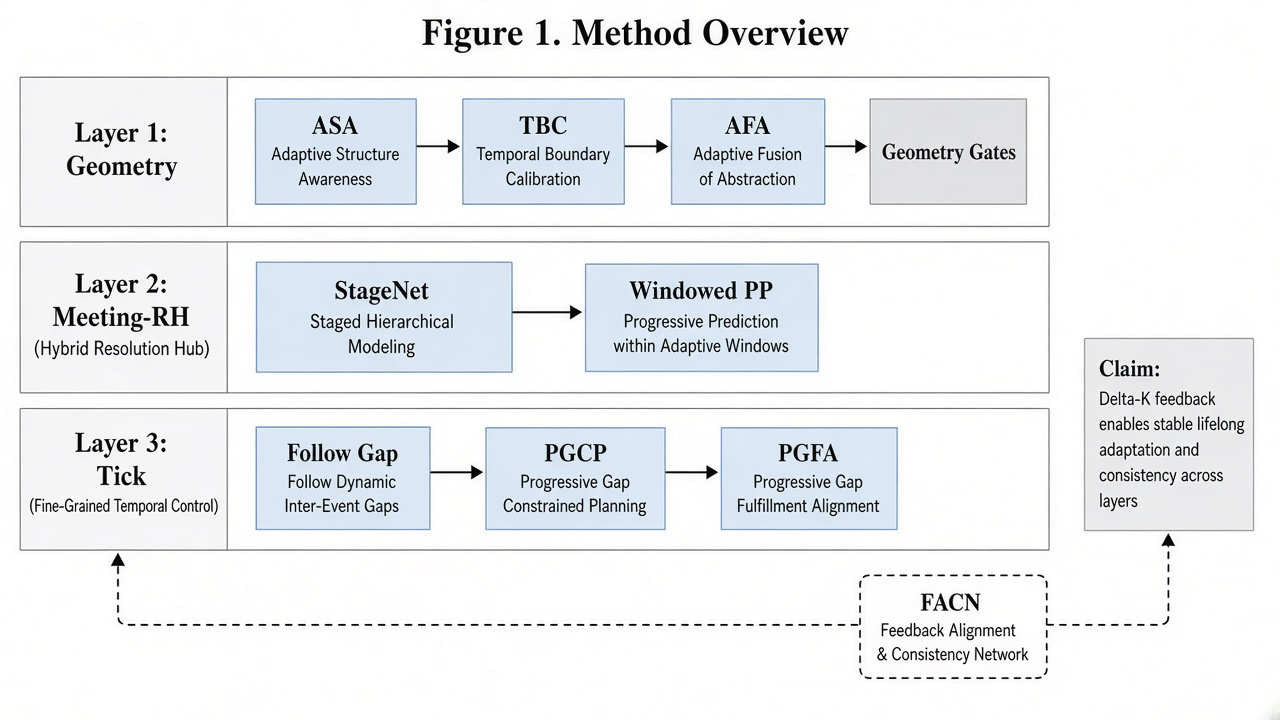
\includegraphics[width=0.95\linewidth]{../figures/fig1_overview.jpg}
\caption{Meeting-RH stack: geometry gates, meetings, tick execution, and FACN feedback on $K$.}
\label{fig:overview}
\end{figure}

\begin{figure}[t]
\centering
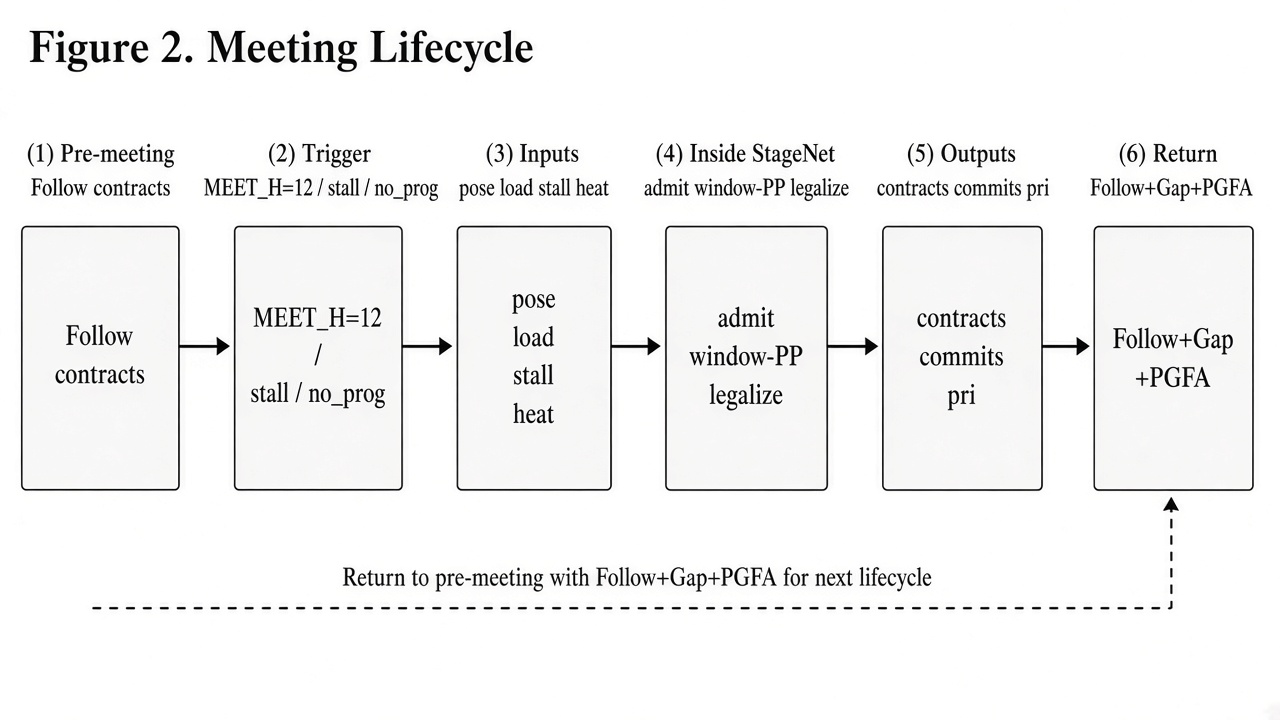
\includegraphics[width=0.95\linewidth]{../figures/fig2_meeting.jpg}
\caption{Meeting lifecycle: pre-follow $\to$ trigger $\to$ inputs $\to$ internal steps $\to$ contracts.}
\label{fig:meeting}
\end{figure}

\section{Experiments}
\subsection{Setup}
Baselines: PIBT, M0 (space-time A* + greedy assign), PP (priority allocation + space-time A*), windowed ECBS, Hier (M0 easy / ECBS hard). Ours: Meeting-RH + protocols + StageNet (ASA) + FACN (AFA). Seed: \texttt{PYTHONHASHSEED=0}; CPU; per-map subprocesses.

\subsection{Main results}
\begin{table}[t]
\centering
\caption{Aggregate results on SH01--20 (official 100). Lower sim/wall is better among VALID$\land$full100. $^\dagger$sim on incomplete maps is not comparable as ``faster.''}
\label{tab:main}
\begin{tabular}{lccccc}
\toprule
Method & full100 & VALID & avg\_done & avg\_sim & avg\_wall \\
\midrule
PIBT & 8/20 & 20/20 & 63.9 & 62811 & 40.5s \\
M0 & 4/20 & 20/20 & 44.6 & 942$^\dagger$ & 1478s \\
PP & 1/20 & 7/20 & 32.4 & 848$^\dagger$ & 1716s \\
ECBS & 20/20 & 20/20 & 100 & 7364 & 543s \\
Hier & 20/20 & 20/20 & 100 & 4018 & 1032s \\
\textbf{Ours} & \textbf{20/20} & \textbf{20/20} & \textbf{100} & \textbf{1708} & \textbf{$\sim$28s} \\
\bottomrule
\end{tabular}
\end{table}

Among methods with 20/20 full100, Ours reduces avg\_sim to $\sim$42\% of Hier and $\sim$23\% of ECBS, with wall-clock $\sim$28s vs.\ hundreds--thousands of seconds. Protocol-only vs.\ legacy FULL: $\approx\!-9.0\%$ avg\_sim, 0 worse maps. FACN v2 vs.\ noFACN (SH01--40): $\approx\!-5.82\%$ avg\_sim (20/13/5 better/same/worse).

\subsection{Ablations}
Without StageNet: hard maps collapse (SH10 done 60; SH17 done 32). Without PGCP tools: SH10/11/12/17 completion drops. Without PGFA: SH17 done 20; SH03 sim inflates. Without FACN: open large fleets hurt (SH20 sim $660\!\to\!813$). Global direction-field nets are not in the default stack.

\begin{figure}[t]
\centering
\begin{subfigure}{0.48\linewidth}
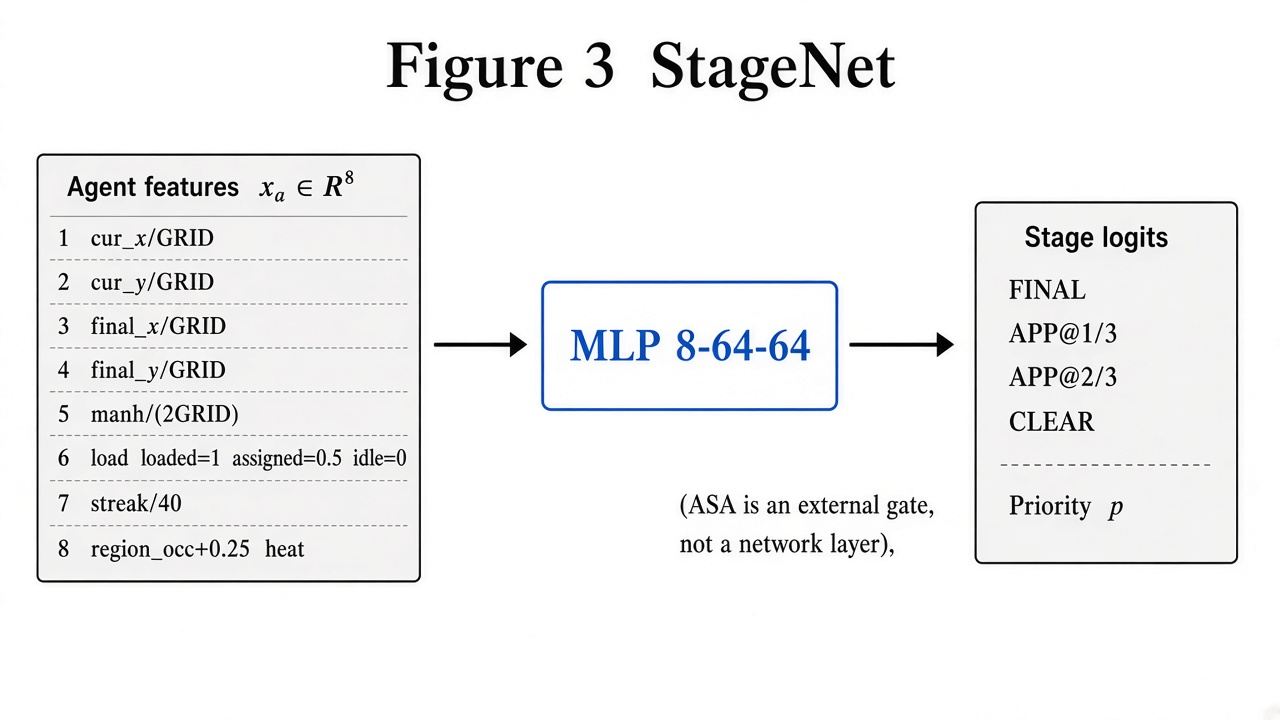
\includegraphics[width=\linewidth]{../figures/fig3_stagenet.jpg}
\caption{StageNet I/O.}
\end{subfigure}
\hfill
\begin{subfigure}{0.48\linewidth}
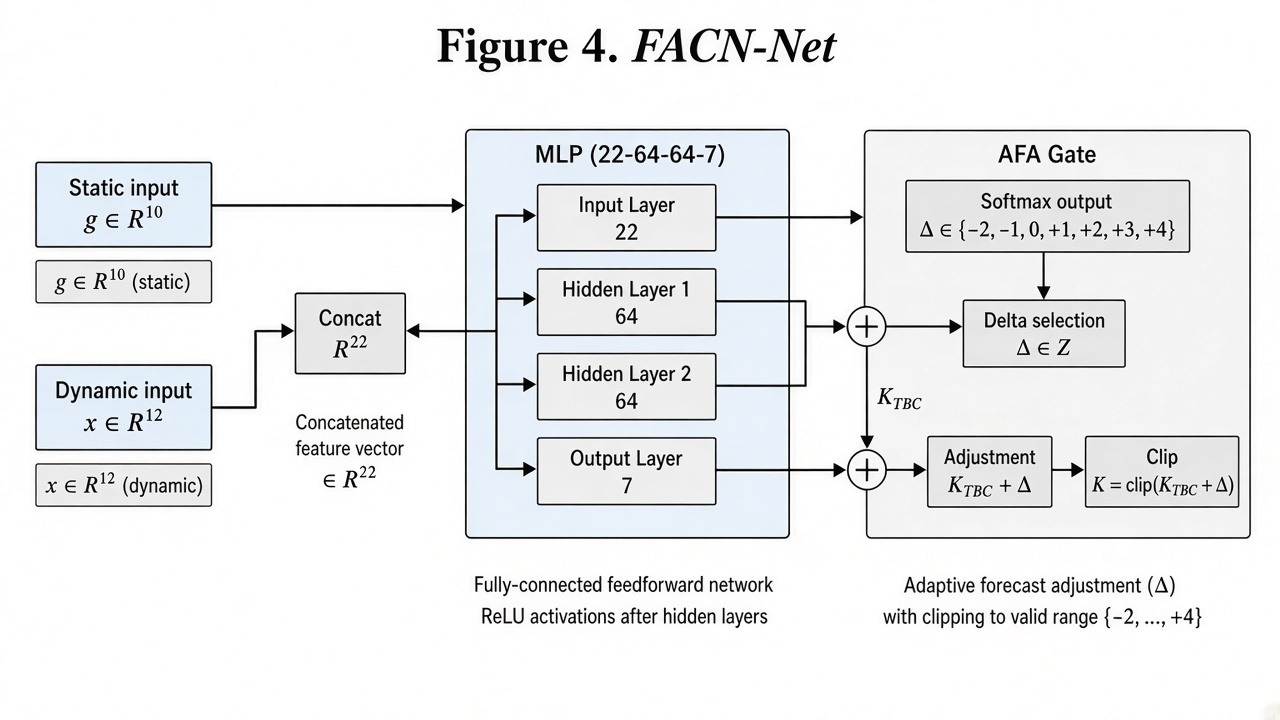
\includegraphics[width=\linewidth]{../figures/fig4_facn.jpg}
\caption{FACN I/O.}
\end{subfigure}
\caption{Small imitation modules used by Meeting-RH.}
\label{fig:nets}
\end{figure}

\subsection{Why windowed BFS beats serial M0 A*}
M0 repeatedly runs \textbf{full-horizon space-time A*} against a dense reservation table. Meeting-RH mostly follows contracts; meetings call \textbf{priority-ordered space-time BFS} only inside $W$, cutting call frequency, depth, and thrash.

\section{Limitations}
Incomplete relative to CBS; FACN held-out generalization is limited; protocols interact; stress maps $\neq$ industrial digital twin; fixed seeds/CPU.

\section{Conclusion}
Meeting-RH couples geometry-gated protocols with StageNet and FACN for explainable lifelong MAPD. Empirically it matches strong search baselines on validity and completion while improving simulation time and wall-clock. Future work: stronger held-out concurrency learning and tighter integration with anytime windowed search~\citep{li2021mapflns}.

\bibliographystyle{plainnat}
\bibliography{../refs}

\end{document}
